\chapter{Pojmy v kontextu této práce}\label{sec:terms} %PROVED
V této kapitole definujeme základní pojmy v kontextu této práce. Pojmy, jako kompetence, často nemají jen jednu definici, proto je nutné vybrat právě tu, v jejíž souvislosti budeme daný pojem používat. Ve většině případů se jedná o stručné definice, někdy je však potřeba pojem definovat podrobně a zmínit i další okolnosti.
\section{Kompetence}
Pojem kompetence se vyskytuje v literatuře hned v několika významech. Dva nejdůležitější jsou: kompetence ve smyslu oprávnění a kompetence ve smyslu schopnost. Oba významy jsou si velmi podobné.\par
První význam je dostupný např. v českém slovníku cizích slov. Tento slovník mimo jiné uvádí, že kompetence je definována jako pravomoc nebo rozsah pravomocí.\cite{cite:06}\par
Druhý význam, který uvádí Cambridge dictionary je následující: Kompetence je schopnost osoby vykonat danou činnost správně (tj. uspokojivě popř. efektivně) \cite{cite:01} (překlad autor).\par
První případ, tedy kompetence ve smyslu oprávnění, se v našem případě nehodí. Zkoumáme totiž více kompetence ve smyslu způsobilosti v rámci nabitých dovedností a znalostí, nikoliv získaných oprávnění. Na druhou stranu oprávnění člověk často nabývá na základě svých znalostí a dovedností, takže jsou si významy opravdu velmi blízké. Přesto v této práci vezmeme za svou druhou definici.\par
Z upřednostněné definice plyne, že kompetence vždy souvisí s danou činností - tu nazveme předmětem kompetence. Dále si ještě definujeme slovní spojení \textit{být kompetentní}. Tím navážeme na samotnou definici kompetence. Být kompetentní znamená: Mít schopnost vykonat danou činnost správně (tj. uspokojivě, efektivně).\par
Poslední pojem spojený s kompetencemi je míra kompetence. Míra kompetence je metrika vyjadřující, jak moc je osoba kompetentní.
\subsection{Složení kompetencí}
Každá osoba má sadu svých kompetencí podmíněnou mnoha faktory. Menší část těchto faktorů lze poměrně jednoznačně (i když složitě) popsat~-~obr.~č.~\ref{fig:competence_structure}, část nad hladinou ledovce, tedy znalosti a dovednosti. Naproti tomu větší část, bližší k osobnosti člověka a jeho vnitřnímu vnímání, je velmi těžké popsat a získat~-~obr.~č.~\ref{fig:competence_structure}, část pod hladinou ledovce.
\begin{figure}[htbp!]
	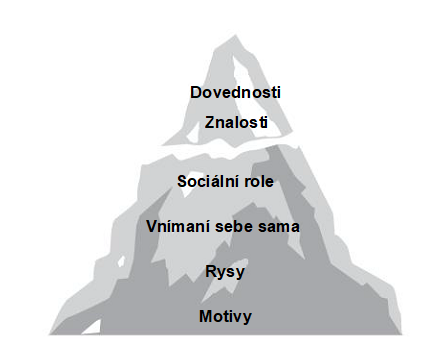
\includegraphics[width=0.65\linewidth]{competence_structure.png}
	\caption{Složení kompetencí znázorněná pomocí ledovce (zdroj \cite{cite:02})}
	\label{fig:competence_structure}
\end{figure}

\section{Znalosti a dovednosti}
Znalosti a dovednosti jsou ze všech složek  kompetencí nejlépe uchopitelné. To však není, vzhledem k jejich komplexnosti, nijak uspokojivé. Důvodem je, že u nich lze předpokládat, že je buď sám vlastník umí popsat, nebo je možné je poměrně jednoznačně vyčíst z jeho činů (např. z jeho vědeckých prací, z potvrzených referencí zaměstnavatelem). Na rozdíl od rysů, motivů a sociálních rolí (obr. č. \ref{fig:competence_structure}), které ani samotný vlastník často nedokáže přesně definovat.\par
Je tedy velmi pravděpodobné, že optimální cesta za vyhledáváním dle kompetencí povede okolo znalostí a dovedností. Pro začátek si je definujeme.
\subsubsection*{Znalost}
 Pochopení určité informace, které osoba získá zkušeností nebo studiem. \cite{cite:01} (přeložil autor) \par
\paragraph{Typy znalostí:}
\begin{itemize}
\item Deklarativní
\begin{itemize}
\item Popisují, jaké věci známe a co o nich víme; např. pes je zvíře, pes má ocas
\item Mohou být popsány pomocí grafů a podobných struktur
\end{itemize}
\item Procedurální
\begin{itemize}
\item Popisují, jak věci fungují, např. jestliže je pes hladový, najde si jídlo a sní ho
\item Mohou být popsány pomocí pravidel \cite{cite:11}
\end{itemize}
\end{itemize}
Znalosti ještě v kontextu jejich vyvozování dělíme na \textit{explicitní} a \textit{implicitní}.  \textit{Explicitní} znalosti jsou znalosti, které byli objektu (počítači, osobě) přímo sděleny, libovolnou formou. \textit{Implicitní} znalosti je poté objekt schopen sám vyvodit na základě znalostí explicitních (např. pomocí logiky).\cite{Stephan2007}\par
Často používaným pojmem je \textit{znalostní báze}, která se nejčastěji pojí k nějakému seskupení lidí, komunitě, popř. k jinému jednotícímu prvku. V podstatě se jedná o množinu znalostí a jejich propojení, které se vztahují ke zvolené jednotící entitě např. firmě, vědeckému výzkumu, nebo i k určitému vědnímu oboru. Například součástí znalostní báze oboru informatika by mohly být všechny známé pojmy s jejich definicemi, propojené různými sémantickými vazbami (nadřazenost, podřazenost, souvislost a jiné).
\subsubsection*{Dovednost}
Dovednost je učením a praxí získaná dispozice ke správnému, kvalitnímu, rychlému a úspornému vykonávání určité činnosti vhodnou metodou \cite{cite:03}. Jinými slovy je to schopnost využít znalosti efektivně k vykonávání určité činnosti \cite{cite:04}.
\section{Další pojmy}
\subsection*{Osoba}
V kontextu této práce je osoba jakýkoliv člověk.
\subsection*{Pracoviště}
Pracoviště je v kontextu této práce seskupení osob. Obvykle má název, místo působení a vedoucí osobou. Dále se dělí na týmy, které pracují společně na cílech definovaných vedoucím.\par
V této práci pojednáváme o vyhledávání osob a pracovišť dle kompetencí. Proto je nutné definovat, co znamená pojem kompetence pracoviště. Pracoviště je kompetentní k určitému předmětu kompetence v případě, že je kompetentní osoba, která je jeho součástí. Váha dané kompetence pracoviště je potom určena součtem váh dané kompetence přes všechny osoby na daném pracovišti.
\subsection*{Data}
Fakta či fikce zapsané v čitelné podobě, čitelné pro stroje či lidi.
\subsection*{Informace}
Informace jsou data o něčem nebo o někom. Jinými slovy jsou to data, která mají daný význam.
% \subsection*{Databáze kompetencí}
% Systém pro ukládání pracovišť, osob a jejich kompetencí, navržený takovým způsobem, který optimálně vyhovuje pozdějšímu efektivnímu zpracování těchto dat (např. vhodná reprezentace). Zpracováním je myšleno: vytváření, čtení (vyhledávání), editace, mazání.\par
% Databáze kompetencí musí mít vždy pevně definovanou množinu osob, kteří se v ní nacházejí (např. zaměstnanci konkrétní organizace, vědecké týmy, akademičtí pracovníci).
\subsection{Jazyk} \label{sec:jazyk}
Obecný jazyk definujme jako prostředek komunikace mezi dvěma a více objekty, nebo jejich částmi. Jazyk je používán k reprezentaci informací.
\subsubsection*{Přirozený jazyk}
Znaky, symboly, zvuky a metody předávání informací, pocitů nebo nápadů.\cite{cite:05} Tento jazyk se vyvinul postupně a přirozeně jako způsob komunikace mezi lidmi.\cite{cite:07}  
\subsubsection*{Formální jazyk}
Tento jazyk je určený pro situace, kdy přirozený jazyk nestačí např. v matematice, logice a informatice. Symboly a vzorce mají mezi sebou přesně definované syntaktické a sémantické vztahy. \cite{cite:07}\par
Přesná syntaxe a sémantika jsou důvodem, proč jsou tyto jazyky obecně v oborech jako je informatika upřednostňovány. Na rozdíl od přirozeného jazyka není formální jazyk tolik zatížen následujícími vlastnostmi:
\begin{itemize}
\item \textbf{Nejednoznačnost} - formální jazyky jsou navrhovány tak, aby buď minimálně nebo vůbec neobsahovali nejednoznačné symboly a vzorce
\item \textbf{Redundance} - pro vyrušení nejednoznačnosti přirozené jazyky zapojují redundanci (popisují jednu skutečnost více způsoby); formální jazyky se tomuto vyhýbají a díky tomu jsou stručnější
\item \textbf{Literárnost} - ve formálních jazycích neexistují idiomy, metafory a podobné jevy \cite{cite:08}
\end{itemize}
Výše zmíněné vlastnosti obvykle přirozený jazyk má, tím pádem je obtížně použitelný v informatice, matematice a podobných oborech.
\section{Shrnutí}
Na první pohled se může zdát, že vysvětlené pojmy spolu příliš nesouvisí. Později se v této práci budeme k některým zmíněným pojmům vracet, případně je budeme již jen používat. Přestože některé pojmy nezmíníme explicitně, v této kapitole mají své místo, tvoří totiž teoretický podklad pro lepší pochopení celé problematiky.

%TODO obrázek pro ilustraci provázanosti pojmů

%ZBYTKY
% \subsection*{Slovo}
% Základní jednotka přirozeného jazyka. \cite{cite:05}